\documentclass{article}

\usepackage[top=2cm, bottom=2cm, left=2cm, right=2cm]{geometry}
% \pagestyle{headings}

\usepackage[francais]{babel}
\usepackage[T1]{fontenc}
% \usepackage[latin1]{inputenc} %windows
\usepackage[utf8x]{inputenc} %linux

\usepackage{soul}
\usepackage{amsmath}
\usepackage{amssymb}
\usepackage{mathrsfs}
\usepackage{wrapfig}
\usepackage{graphicx}

\title{Module ADC : Classification supervisée \\ Devoir maison -- Seconde partie}
\date{vendredi 19 décembre 2014}
\author{Simon \bsc{Besson-Girard} & Nicolas \bsc{Wattiez}}
%%%%%%%%%%%%%%%%%%%%%%%%%%%%%%%%%%%%%%%%%%%%%%%%%%%%%%%%%%%%%%%%%%%%%%%%
% BEGIN DOCUMENT
%%%%%%%%%%%%%%%%%%%%%%%%%%%%%%%%%%%%%%%%%%%%%%%%%%%%%%%%%%%%%%%%%%%%%%%%
\usepackage{Sweave}
\begin{document}
\maketitle

\paragraph{Avant toutes choses,} certaines commandes requièrent 
l'import de librairies. Pour ce 
faire, faites les commandes suivantes dans l'invité de commande 
$\mathtt{R}$:
\begin{Schunk}
\begin{Sinput}
> install.packages("kernlab")
> install.packages("ROCR")
> install.packages("plotrix")
> library(MASS)
> library(kernlab)
> library(ROCR)
> library(plotrix)
\end{Sinput}
\end{Schunk}

Pour une raison qui nous est inconnue, il est déconseillé de 
copier-coller tout le script (fichier .R attaché) en une seule fois. Des
 erreurs de compilation pourraient apparaitre. Il est recommandé 
 d'utiliser la fonction $\mathtt{source("script.R")}$.
 
%%%%%%%%%%%%%%%%%%%%%%%%%%%%%%%%%%%%%%%%%%%%%%%%%%%%%%%%%%%%%%%%%%%%%%%%
% SECTION 5
%%%%%%%%%%%%%%%%%%%%%%%%%%%%%%%%%%%%%%%%%%%%%%%%%%%%%%%%%%%%%%%%%%%%%%%%
\section{Utilisation des machines à vecteurs supports}
\paragraph{5.1.}Fonction $\mathtt{SVM.accuracy.wrt.C(d)}$ qui trace, 
pour un ensemble d'apprentisage $\mathtt{d}$, le taux d'erreur en 
validation croisée des SVMs sur un jeu de données en fonction du 
paramètre $\mathtt{C}$:
\begin{Schunk}
\begin{Sinput}
> SVM.accuracy.wrt.C <- function(d) {
+ 	C.values <- sapply(c(seq(-10,10,le=40)), function (x) 2^x)
+ 	svm.cross <- sapply(C.values,function(x) cross(ksvm(Y~.,data=d,type='C-svc',
+ 			kernel='vanilladot',C=x,cross=20)) )
+ 	svm.error <- sapply(C.values,function(x) error(ksvm(Y~.,data=d,type='C-svc',
+ 			kernel='vanilladot',C=x,cross=20)) ) 
+ 	plot(C.values,svm.cross,type='o',xlab="Valeurs de C",ylab="Erreur",cex=.5,
+ 			ylim=c(min(c(svm.error,svm.cross)),max(c(svm.cross,svm.error))),log="x",
+ 			main="Erreurs sur un jeu généré par \n generateDifficultDatasetAlt(100,30) avec cross=20")
+ 	points(C.values,svm.error,type='o',col='blue',cex=.5)
+ 	legend(x=.5,y=.4,c("Erreur de validation croisée","Erreur à l'apprentissage"),
+ 			fill=c("black","blue"))
+ }
> SVM.accuracy.wrt.C(generateDifficultDatasetAlt(100,30))#
\end{Sinput}
\end{Schunk}
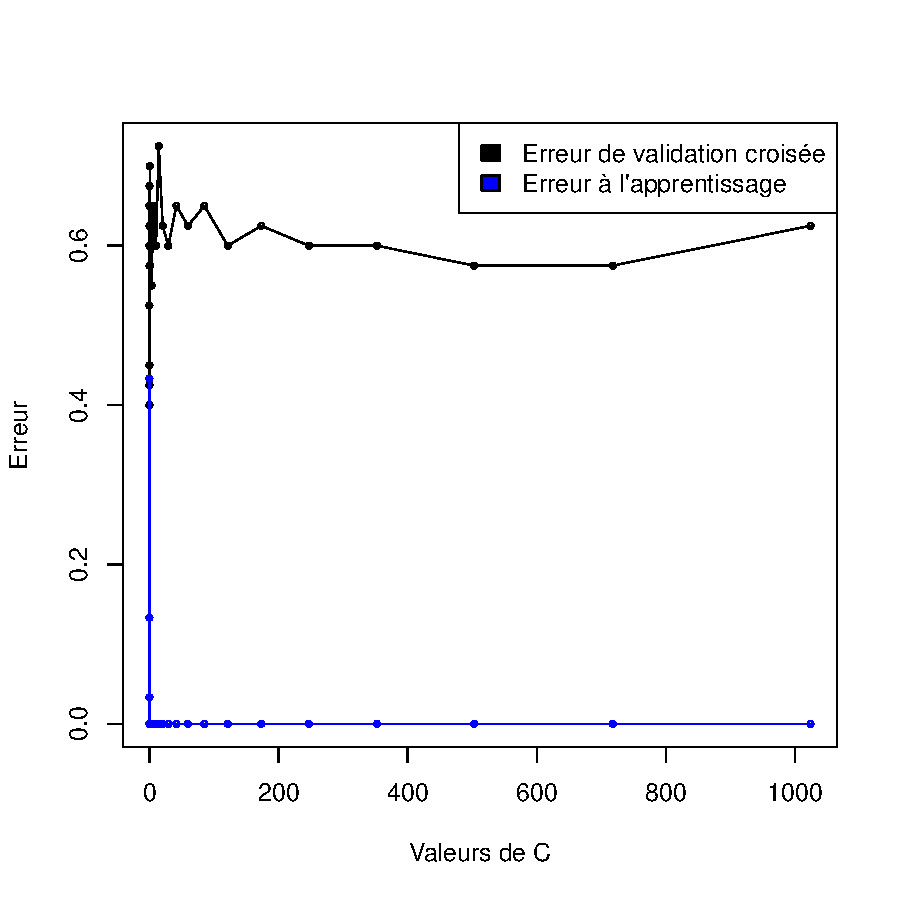
\includegraphics{rapport-SVMaccuracywrtC}
\newline
Commentaire des résultats :
\paragraph{}Plus le nombre de paramètres des vecteurs (dimensions) augmente, plus la 
méthode SVM est efficace. En effet, elle produit toujours le même taux d'erreur, 
quelque soit la valeur du paramètre C choisie, mis à part proche des faibles valeurs.
\paragraph{5.2.}Fonction $\mathtt{selectC(d)}$ qui choisit une valeur de
 $\mathtt{C}$ pour un ensemble d'apprentissage $\mathtt{d}$ :
\begin{Schunk}
\begin{Sinput}
> selectC <- function(d) {
+ 	C.values <- sapply(c(seq(-10,10,le=40)), function (x) 2^x)
+ 	svm.cross <- sapply(C.values,function(x) cross(ksvm(Y~.,data=d,type='C-svc',
+ 			kernel='vanilladot',C=x,cross=20)) )
+ 	svm.error <- sapply(C.values,function(x) error(ksvm(Y~.,data=d,type='C-svc',
+ 			kernel='vanilladot',C=x,cross=20)) ) 
+ 	tab <- as.data.frame(cbind(C.values,svm.cross,svm.error))
+ 	#sur l'ensemble où l'erreur à l'apprentissage est nul, on cherche le minimum 
+ 	#d'erreur de validation croisée
+ 	return(tab$C.values[tab$C.values>1][tab$svm.error==0][tab$svm.cross==min(svm.cross)][1])
+ }
> resultat.selectC <- selectC(generateDifficultDatasetAlt(100,30))
\end{Sinput}
\end{Schunk}
\begin{Schunk}
\begin{Sinput}
> resultat.selectC
\end{Sinput}
\begin{Soutput}
[1] 29.27901
\end{Soutput}
\end{Schunk}
\paragraph{5.3.}Détermination du taux d'erreur moyen de SVMs sur les 
données générées et comparaison avec l'algorithme mediatorHyperplane :
\begin{Schunk}
\begin{Sinput}
> compare.SVM.mH <- function(nbjeux,fonctionquigenere,dimension,taillejeu) {
+ 	f <- function() {
+ 		d <- fonctionquigenere(dimension,taillejeu)
+ 		C.value <- selectC(d)
+ 		error.SVM <- mean(sapply(C.values,function(x) cross(ksvm(Y~.,data=d,type='C-svc',kernel='vanilladot',C=C.value,cross=20))) )
+ 		error.mediatorHyperplane <- error.wrt.n(dimension,taillejeu,fonctionquigenere)[1]
+ 		return(c(error.SVM,error.mediatorHyperplane))
+ 	}
+ 	moyennes <- replicate(nbjeux,f())
+ 	return(list(
+ 		error.SVM = mean(moyennes[1,]),
+ 		error.mediatorHyperplane = (mean(moyennes[2,]))
+ 	))
+ }
> resultat.compareSVM.mH <- compare.SVM.mH(3,generateDifficultDatasetAlt,100,30)